% TikZ 复刻。原图：assets/grating-diffraction.png
% 回退：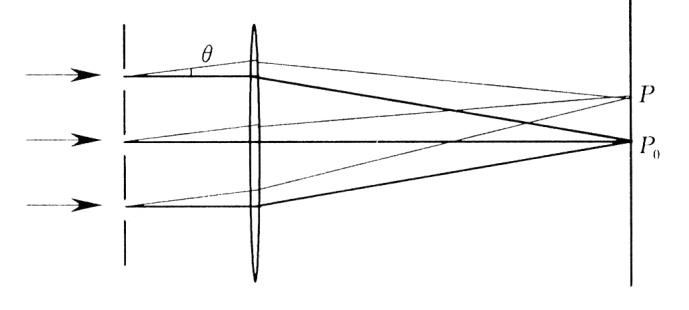
\includegraphics[width=0.88\linewidth]{assets/grating-diffraction.png}
\begin{tikzpicture}[>=Stealth, font=\small]
  \foreach \y in {-1.65,-1.43,...,1.65} {
    \filldraw[fill=gray!70, thick] (-0.08,\y-0.07) rectangle (0.08,\y+0.07);
  }
  \node[above] at (0,1.85) {光栅};
  \foreach \y in {-0.7,-0.23,0.23,0.7} {
    \draw[->, thick] (-3.0,\y) -- (-0.12,\y);
  }
  \node at (-2.1,1.15) {入射光};
  \draw[dashed] (0,-2.05) -- (0,2.05);
  \node[below left] at (0,-1.95) {法线};
  % thin biconvex lens: two shallow arcs, ends do not cross
  \draw[thick] (3.62,-1.55) .. controls (3.80,0) .. (3.62,1.55);
  \draw[thick] (3.88,-1.55) .. controls (3.70,0) .. (3.88,1.55);
  \draw[thick] (3.62,-1.55) -- (3.88,-1.55);
  \draw[thick] (3.62,1.55) -- (3.88,1.55);
  \coordinate (P0) at (7.25,0);
  \coordinate (P) at (7.25,1.12);
  \coordinate (Pp) at (7.25,-1.12);
  \draw[dashed] (0,0) -- (P0);
  \foreach \y in {-0.26,0,0.26} {
    \draw (0.10,\y) -- (3.62,\y) -- (P0);
  }
  \foreach \y in {-0.14,0,0.14} {
    \draw (0.10,\y) -- (3.62,0.72+\y) -- (P);
    \draw (0.10,\y) -- (3.62,-0.72+\y) -- (Pp);
  }
  \fill (P0) circle (1.2pt);
  \fill (P) circle (1.2pt);
  \fill (Pp) circle (1.2pt);
  \node[right] at (P0) {$P_0$ 零级};
  \node[right] at (P) {$P$ $+1$级};
  \node[right] at (Pp) {$P'$ $-1$级};
  % phi 画在光栅右侧、透镜之前，角边落在 +1 级光线上
  \coordinate (O) at (0,0);
  \coordinate (AxR) at (2.95,0);
  \coordinate (RayR) at (2.90,0.58);
  \pic[draw, angle radius=21mm, angle eccentricity=1.22,
       pic text=$\varphi$, pic text options={above}] {angle=AxR--O--RayR};
\end{tikzpicture}
